% -----------------------------------------------------------------------
% Image helper functions

\newcommand{\newImage}[1]{
    \ifIMAGES
        \centering
        \IfFileExists{#1}{\includegraphics{#1}}{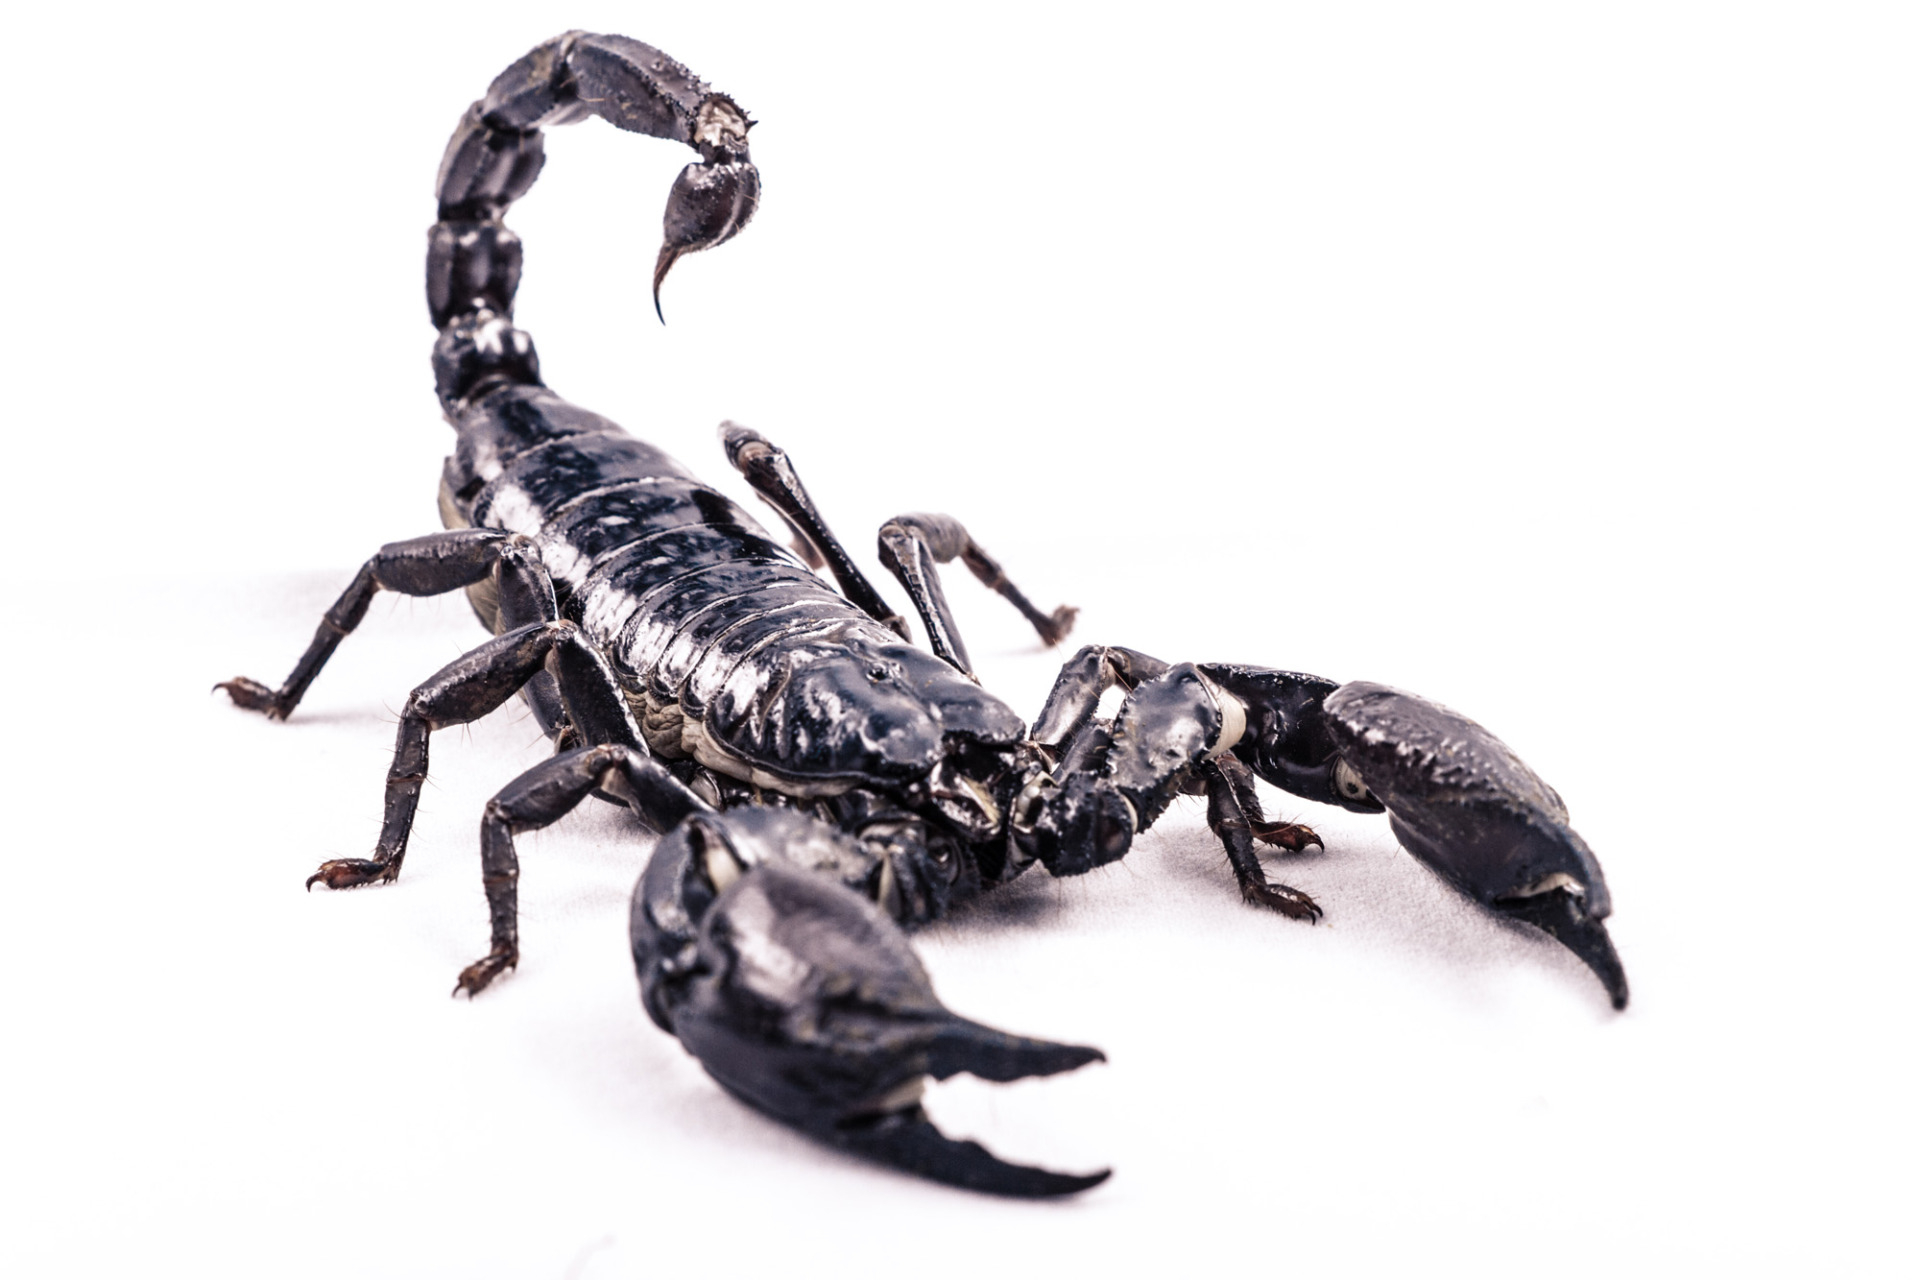
\includegraphics{figures/general/scorpion.jpg}}
    \else
    \fi
}
\newcommand{\newImageResize}[1]{
    \ifIMAGES
        \centering
        \IfFileExists{#1}{
            \resizebox{\textwidth}{!}{
                \includegraphics{#1}
            }
        }
        {
            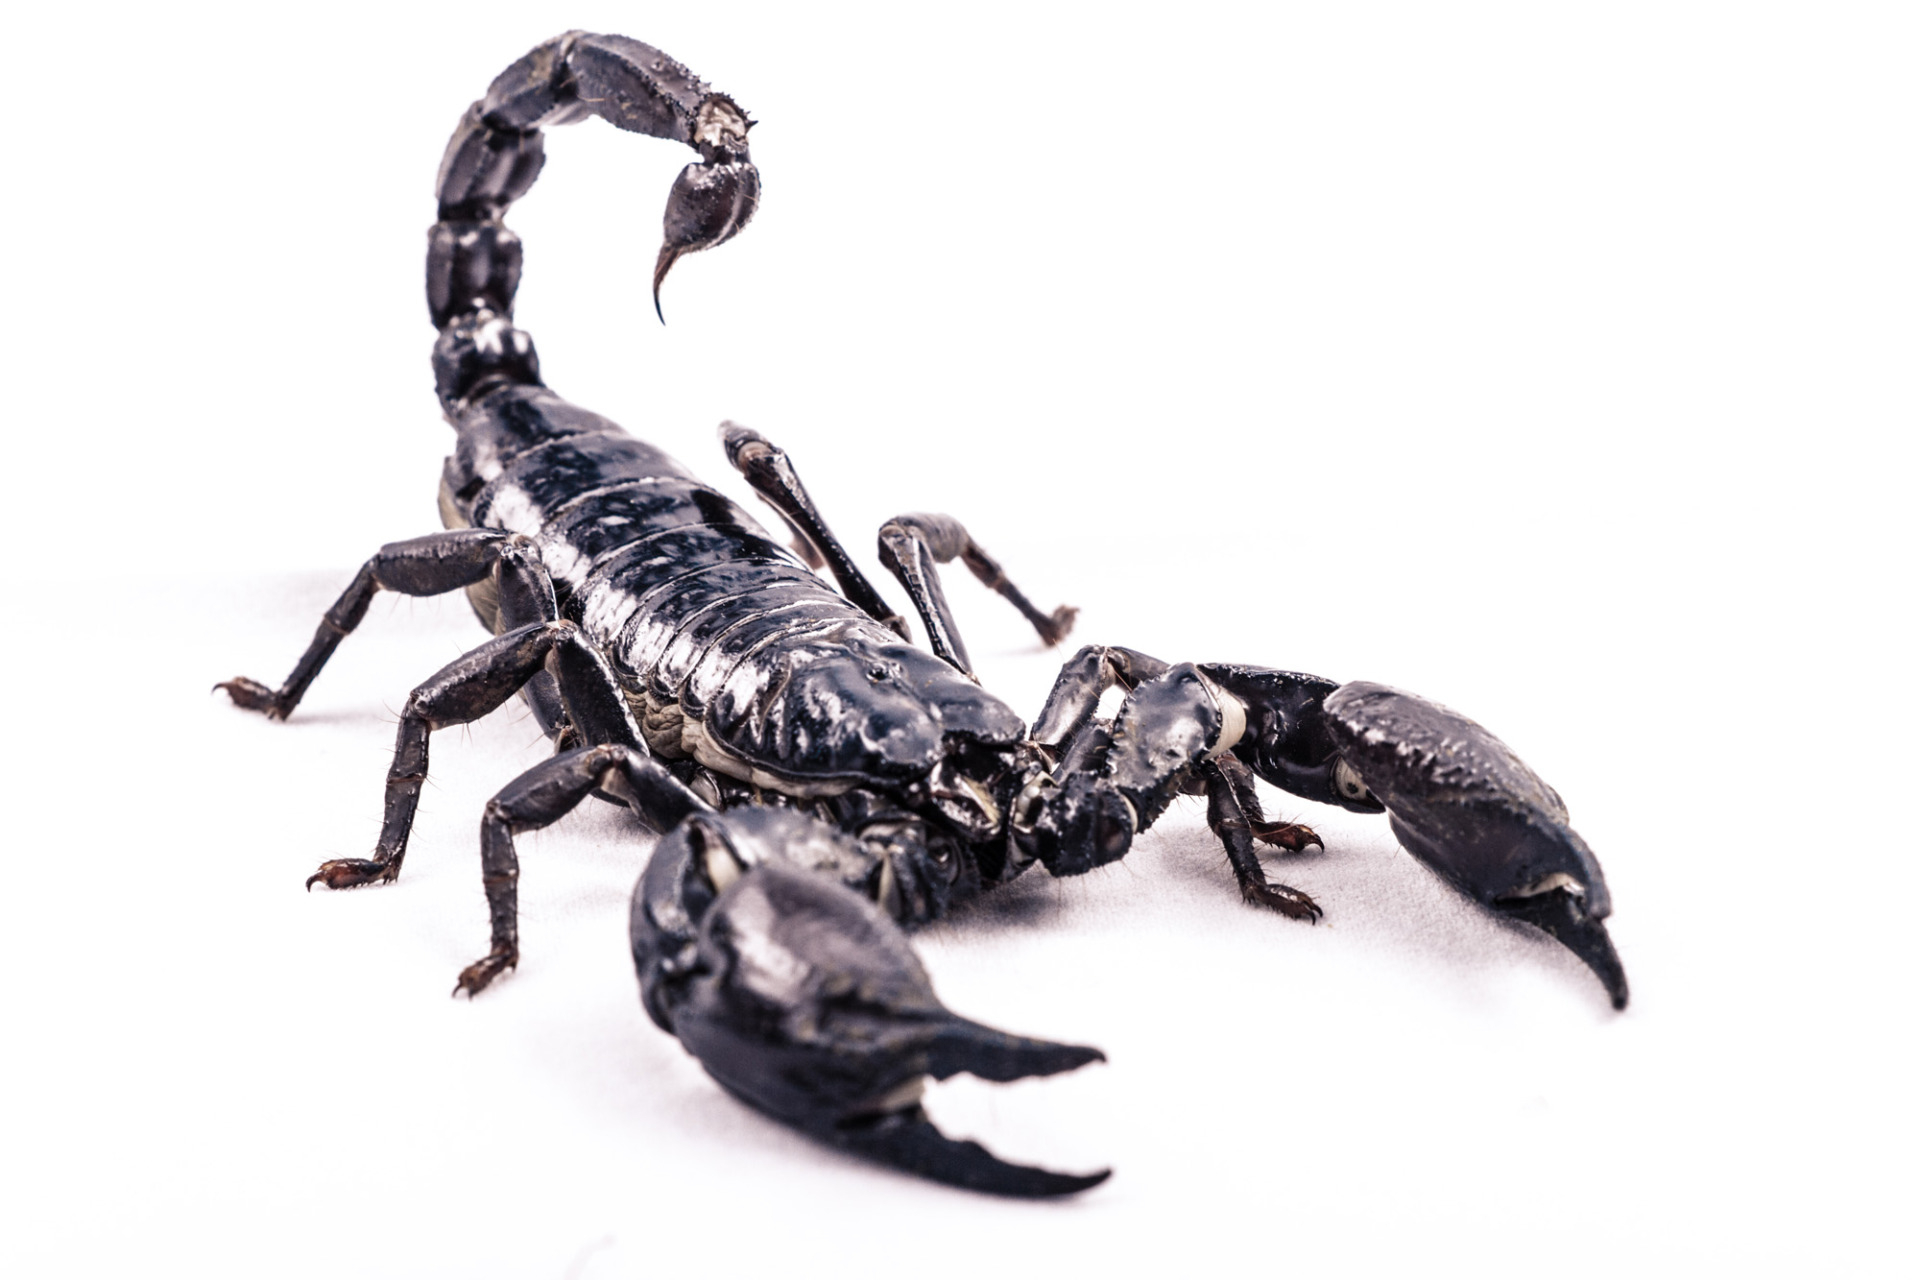
\includegraphics{figures/general/scorpion.jpg}
        }
    \else
    \fi
}
\newcommand{\newImageResizeCustom}[2]{
    \ifIMAGES
        \centering
        \IfFileExists{#2}{
            \resizebox{#1\textwidth}{!}{
                \includegraphics{#2}
            }
        }
        {
            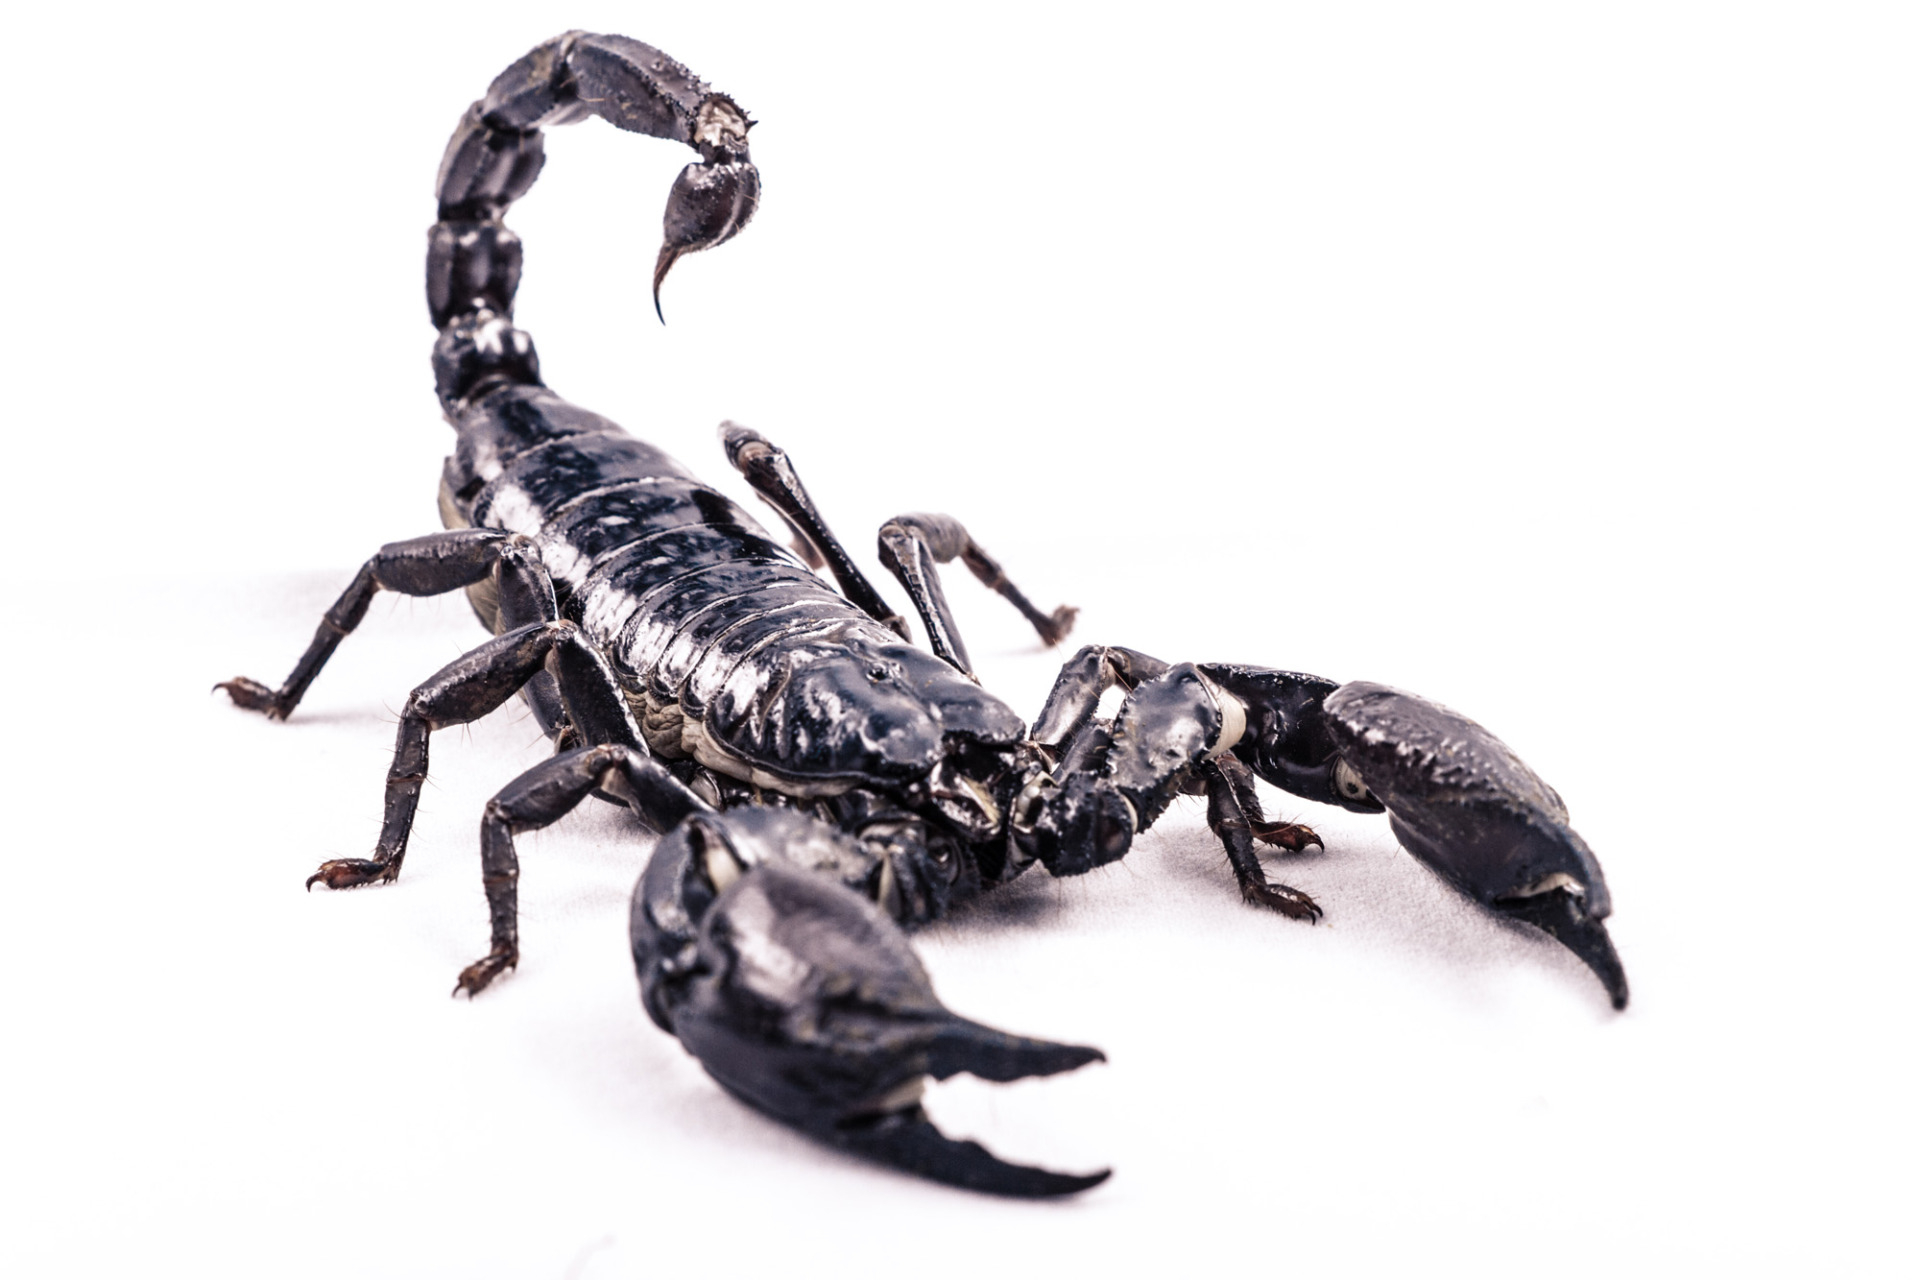
\includegraphics{figures/general/scorpion.jpg}
        }
    \else
    \fi
}
\newcommand{\newImageResizeHalf}[1]{
    \ifIMAGES
        \centering
        \IfFileExists{#1}{
            \resizebox{0.48\textwidth}{!}{
                \includegraphics{#1}
            }
        }
        {
            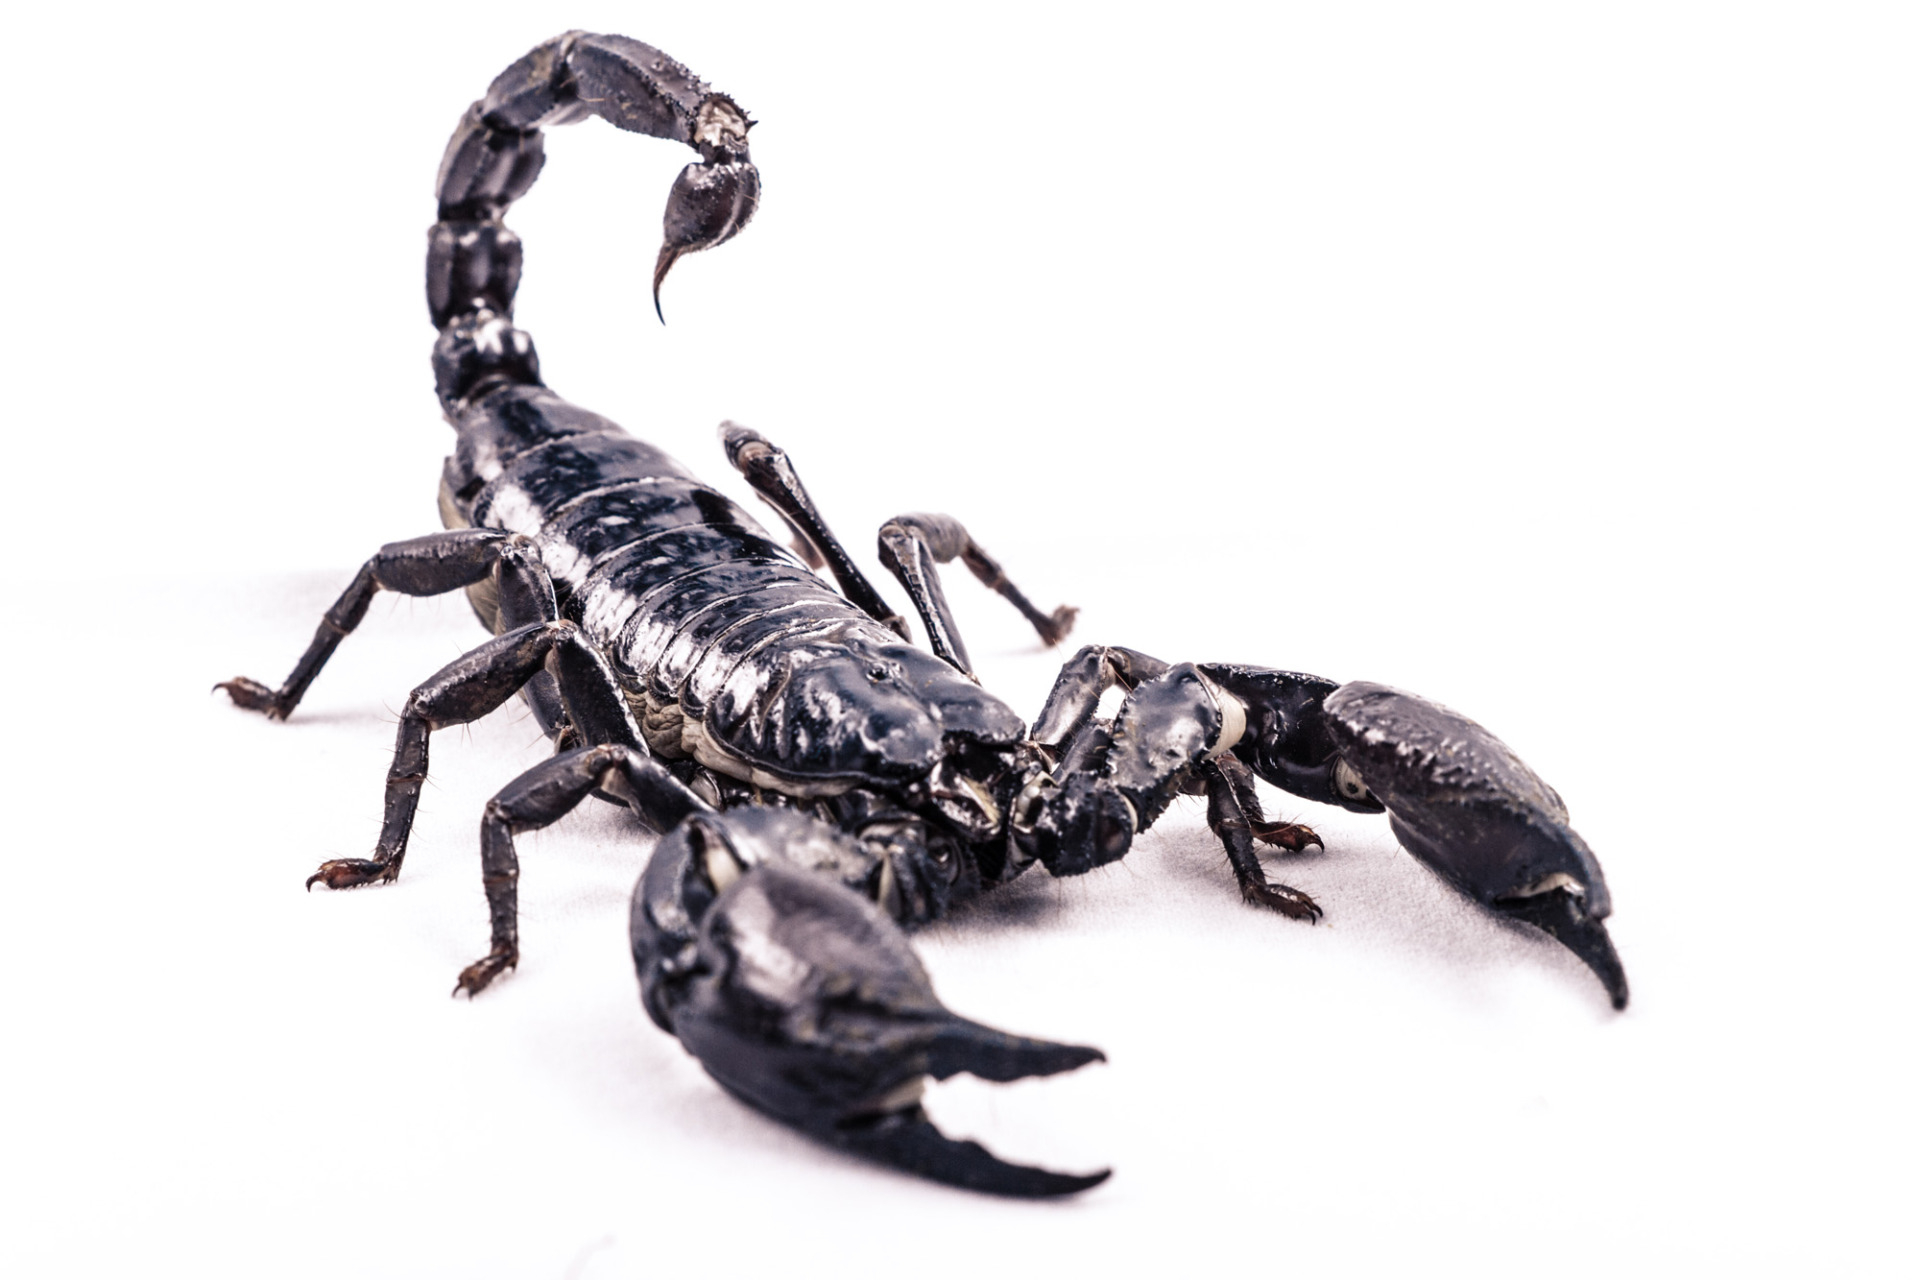
\includegraphics{figures/general/scorpion.jpg}
        }
    \else
    \fi
}
\newcommand{\newImageScale}[2]{
    \ifIMAGES
        \centering
        \IfFileExists{#1}{\includegraphics[scale=#2]{#1}}{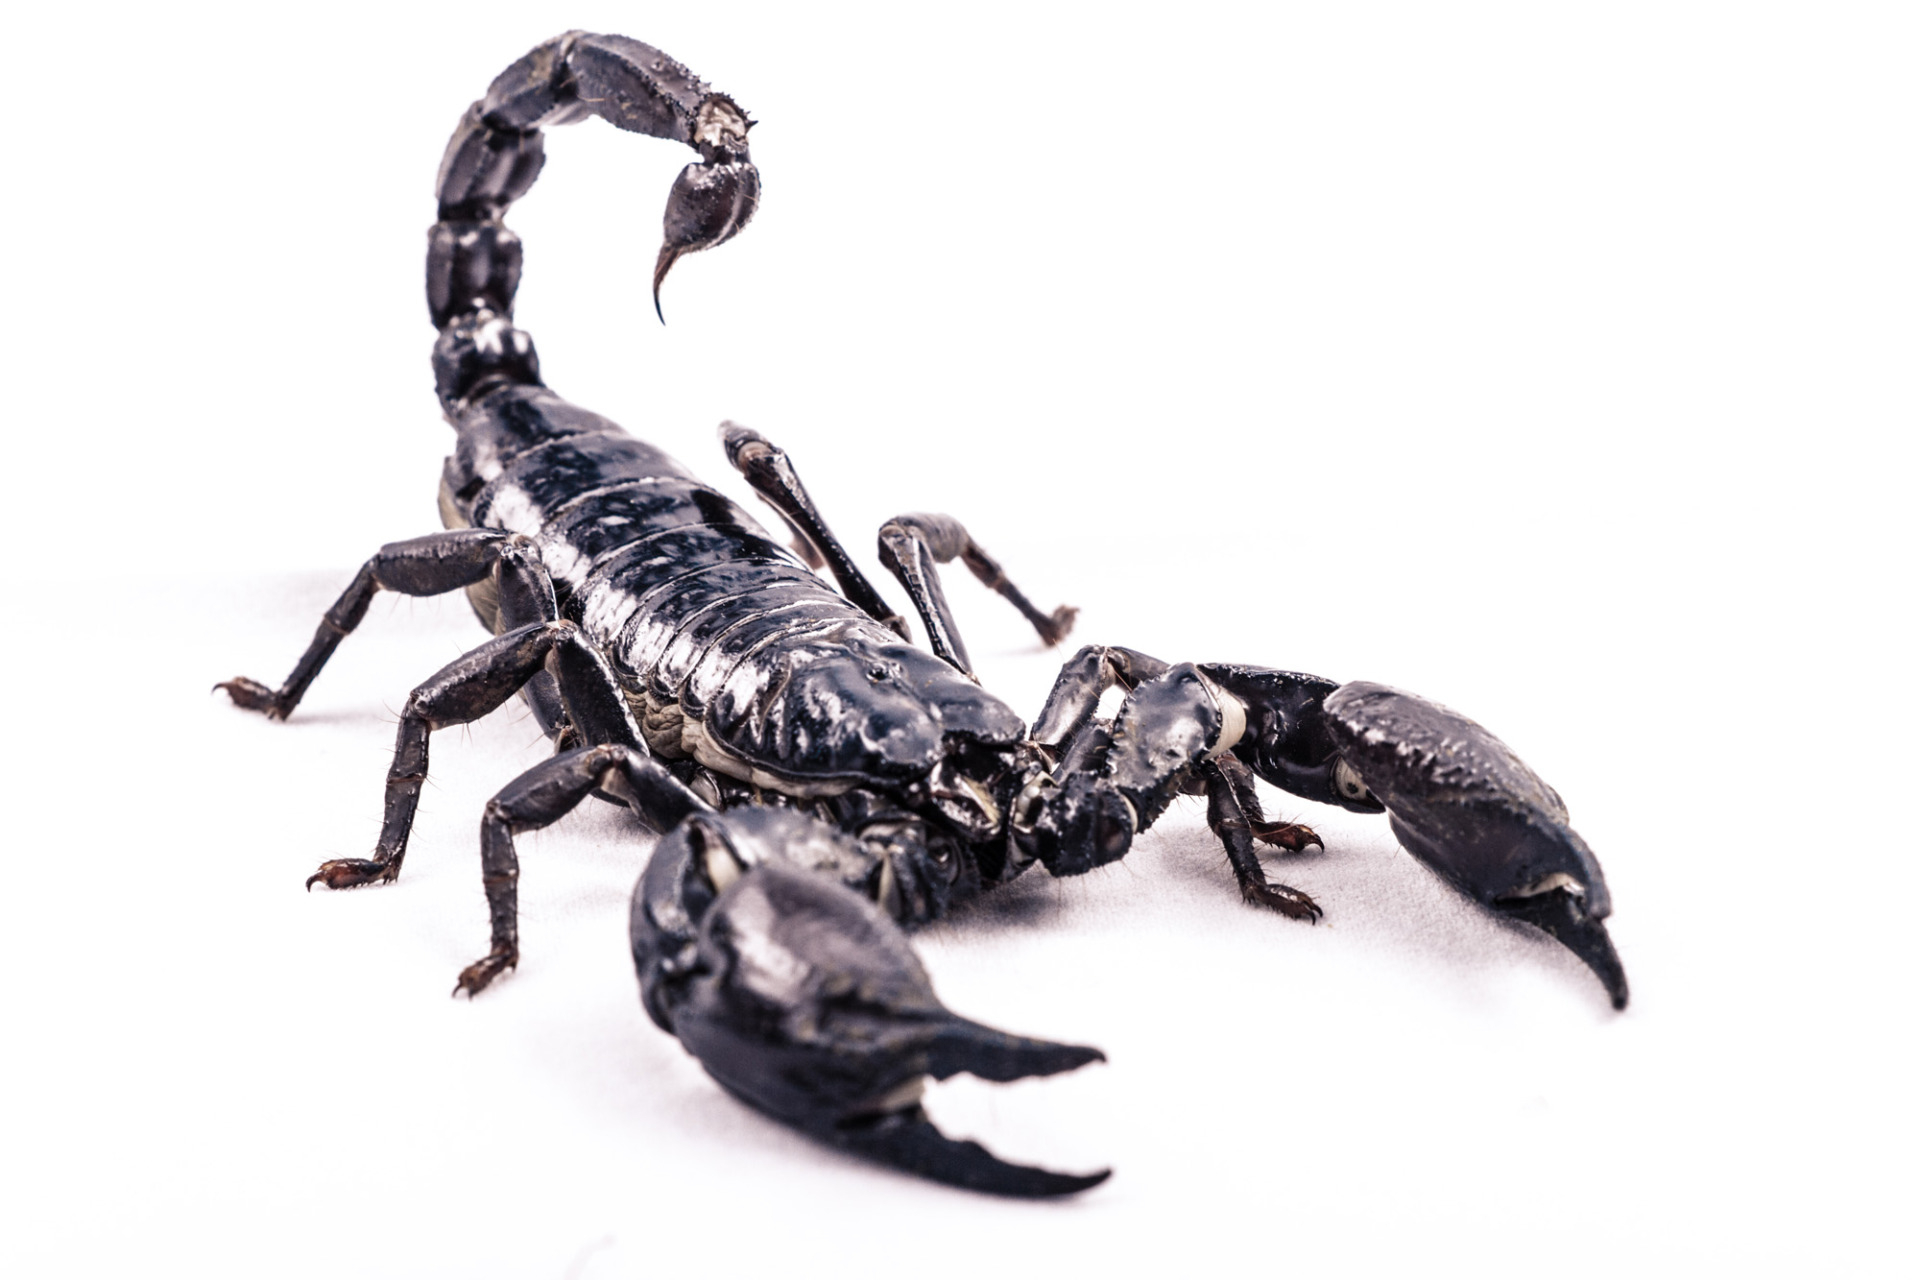
\includegraphics{figures/general/scorpion.jpg}}
    \else
    \fi
}
\newcommand{\newImageScaleRot}[2]{
    \ifIMAGES
        \centering
        \IfFileExists{#1}{\includegraphics[scale=#2,angle=-90]{#1}}{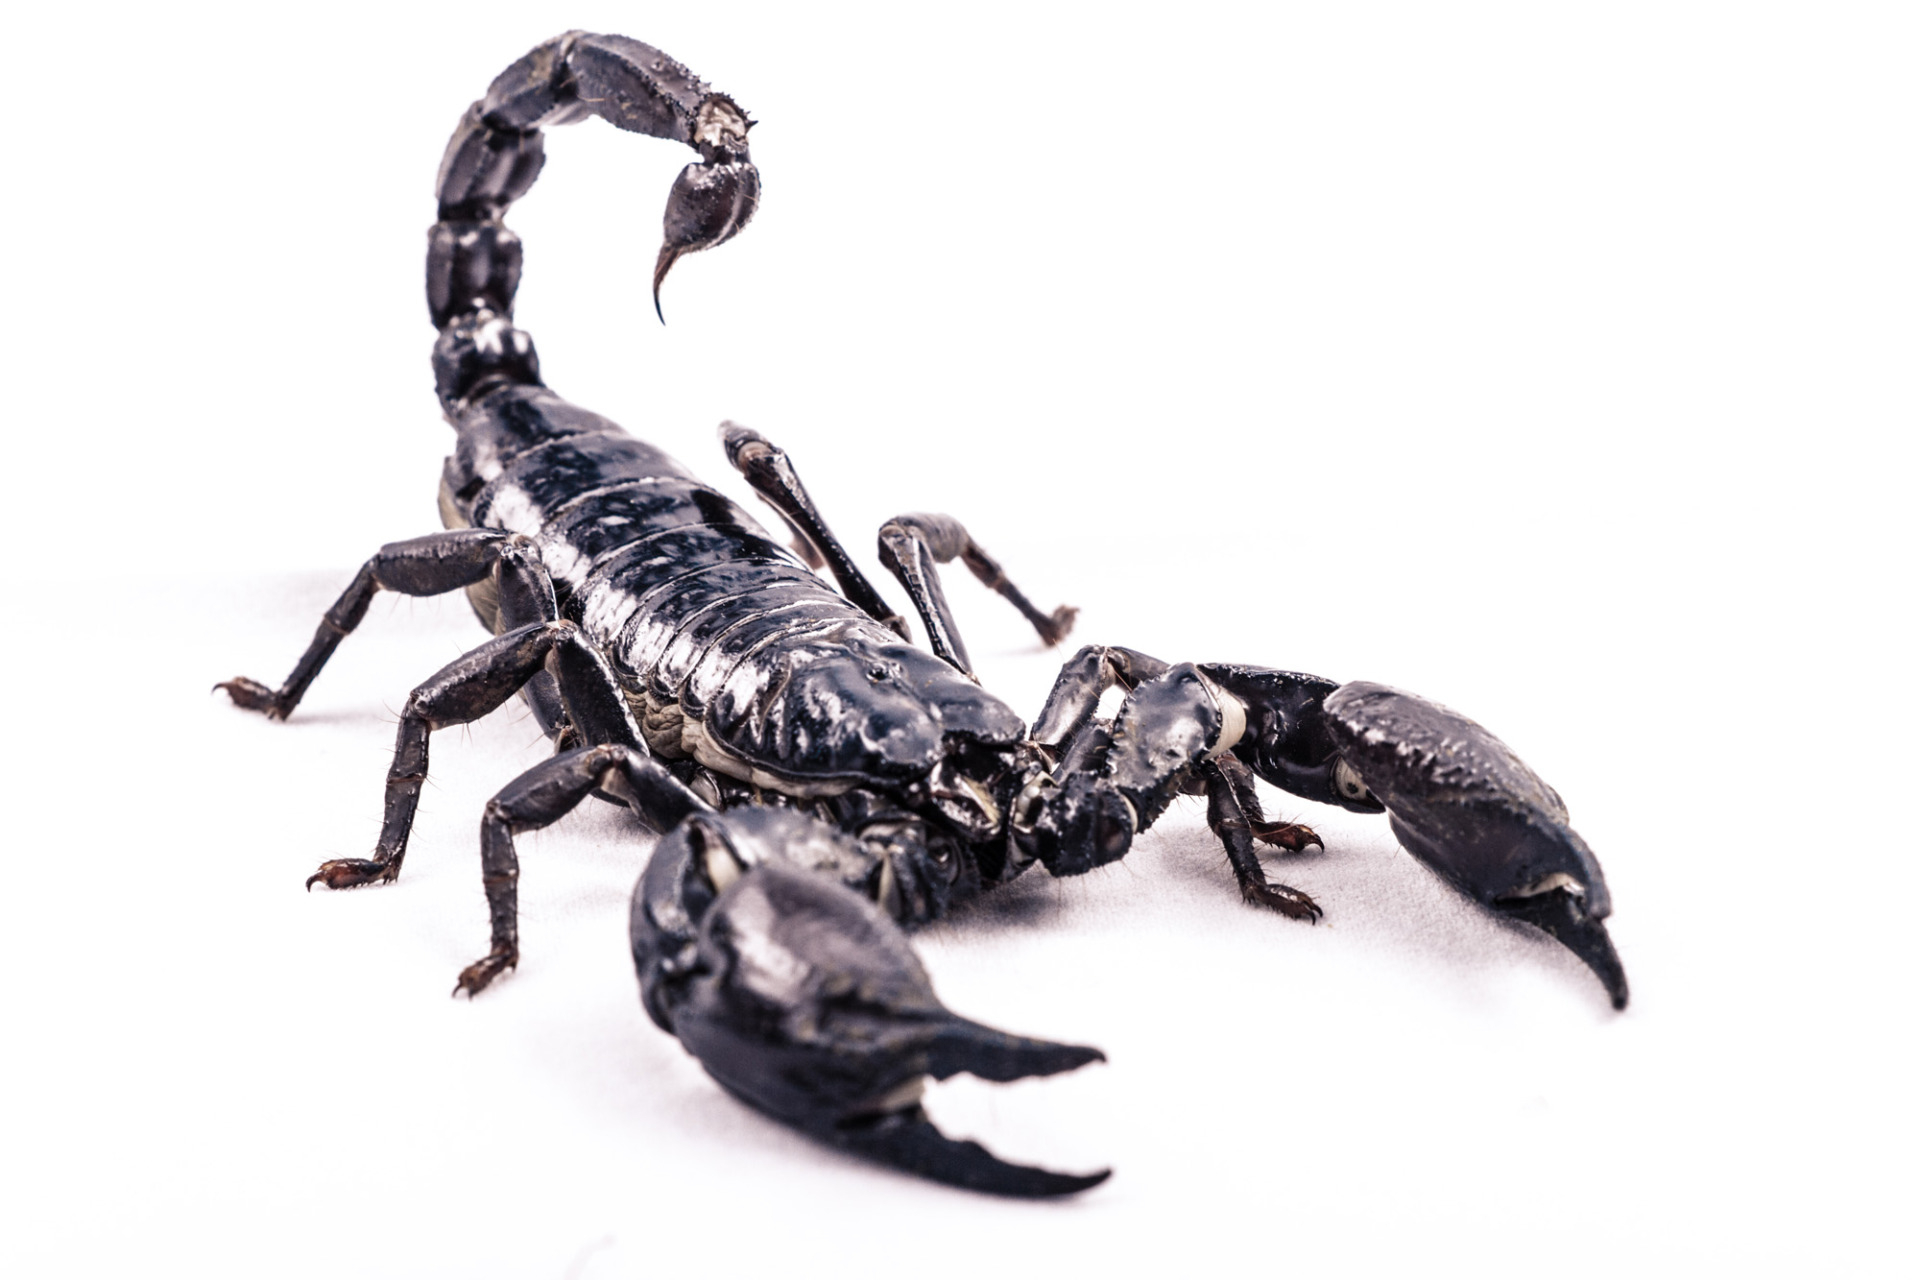
\includegraphics{figures/general/scorpion.jpg}}
    \else
    \fi
}

%---------------------------------------------------
% Equation helpers
\newcommand{\myvec}[1]{\ensuremath{\begin{pmatrix}#1\end{pmatrix}}}
